\section{Classification} \label{sec:classfication}

We addressed the problem of mapping a workload to a standard benchmark class
using two techniques. 
Clustering was our first approach as an unsupervised algorithm seemed to best
fit the data at hand. 
We evaluated the following clustering algorithms in Scikit :

\begin{itemize}
\item \textbf{K-Means} :
This algorithm clusters the samples into groups of similar variance by
minimizing the within-cluster sum-of-squares. The number of clusters
needs to be specified. The algorithms scales well to a large number of
samples.

Given a set of $n$ samples X, the algorithm splits them into $K$ disjoint
clusters, wherein each cluster is defined by the mean $\mu_k$ of the samples in
the cluster i.e. the centroids of the cluster.
The algorithm minimizes the within-cluster sum-of-squares criterion:
$$\sum_{i=0}^{n}\min_{\mu_{k} \in C}(\| x_{k} - \mu_{i} \|^2)$$

\item \textbf{Affinity Propagation}:
This algorithm creates clusters by passing messages between pairs of samples
till it reaches convergence. The clusters are described using a small number of
exemplars that are most representative of the dataset.
The messages indicate the suitability of one sample to be the exemplar of the
other and this gets updated over time for the entire dataset.

For a pair of samples $i$ and $k$, the evidence that sample $k$ should be the
exemplar for sample $i$ is defined by:
$$r(i,k) \leftarrow s(i,k) - max [a(i,j) + s(i,j) \forall j\neq k ]$$

Here, $s(i, k)$ is a similarity metric and availability $a(i, k)$ is the
accumulated evidence that sample $i$ should choose sample $k$ as its exemplar.
Thus, the exemplars chosen are similar enough to many samples and are
chosen by many samples to be representative of themselves.

\item \textbf{Mean-Shift} :
This algorithm tries to identify blobs in a smooth density of samples. 
It works by first identifying candidates for centroids and then filtering them
to eliminate near-duplicates.

For a candidate centroid $x_i$ in iteration $t$, the algorithm updates
the candidate effectively to be the mean of the samples within its neighborhood:

$$x_{i}^{t+1} = x_{i}^{t} + \frac{\sum_{x_{j} \in N(x_i)}K(x_{j} -
x_{i})x_{j}}{\sum_{x_{j} \in N(x_{i})}K(x_{j} - x_{i})} $$

Here, $N(x_i)$ depicts the neighborhood of samples within a given distance
around $x_i$ and the additive term is basically the mean shift vector 
computed for each centroid that points towards a region of the maximum
increase in the density of points.

\item \textbf{Agglomerative Clustering} :
This algorithm is a type of hierarchical clustering algorithms that build nested clusters 
by merging or splitting them successively. 
The cluster hierarchy is represented as a tree, wherein the root is the unique
cluster that gathers all the samples and the leaves are the clusters with only
one sample. 
This particular algorithm uses a bottom up approach. Each samples starts in
its own cluster, and over time the clusters are successively merged together
based on a linkage criteria.
We use the \textit{ward} criteria that minimizes the sum of squared differences 
within all clusters that is effectively a variance-minimizing approach.

\end{itemize}

The clusters found by each algorithm in high-dimensional space are shown in
\cref{fig:clusters}.
We computed standard clustering metrics for each algorithm including the
following :

\begin{itemize}
  \item \textbf{Homogeneity}:
	Given a ground truth, this metric computes if all the clusters contain only
	data points which are members of a single class.
  \item \textbf{Completeness}: 
	Given a ground truth, this metric computes if all the data points that are
	members of a given class are elements of the same cluster.
  \item \textbf{V-measure}: 
	This metric is the harmonic mean between homogeneity and completeness
	\citep{v-measure}.

	$$v = 2 * \frac{(homogeneity * completeness)}{(homogeneity + completeness)}$$

  \item \textbf{Silhouette coefficient}: 
  This metric is computed using the mean intra-cluster distance
  $a$ and the mean nearest-cluster distance $b$ for each sample.
  It is defined for each sample as $(b-a)/max(a, b)$.
\end{itemize}

These results are presented in \cref{fig:clustering-metrics}. We observe that
the clustering algorithms work reasonably well with our dataset.
especially the K-Means and Ward Agglomerative Clustering algorithms. 
Both these algorithms require number of clusters as a parameter. 
However, this is not a restriction for our problem as we know the number of
benchmarks - and hence the number of clusters - that we have.
Algorithms like Affinity-Propagation and Mean-Shift give very high and 
very low estimates for the number of clusters in the dataset.
As we required higher classification accuracy and better intuition about
the classifier, we also experimented with SVM classifiers and decision trees. 
We finally decided to use decision trees as they met both our accuracy
and intuition requirements.

\begin{figure*}[h!]
    \centering
    \fbox{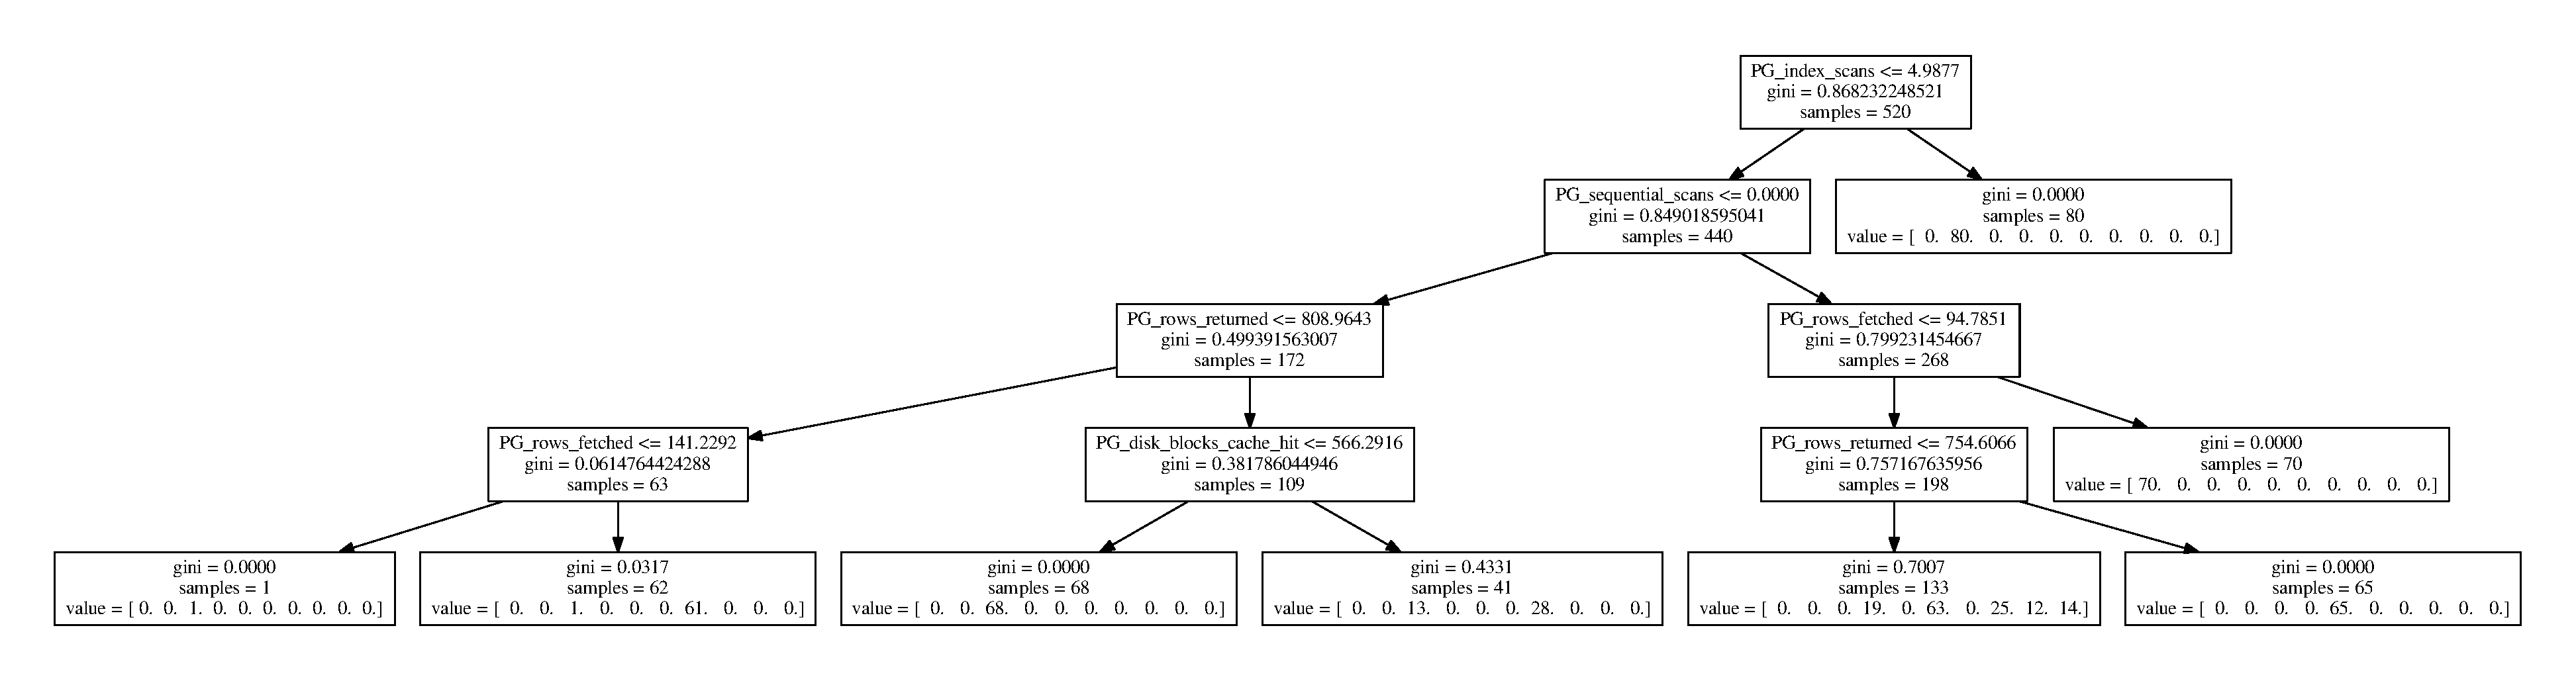
\includegraphics[width=\linewidth]{figure/tree_4.pdf}}
    \caption{Decision tree with max depth set to 4.}
    \label{fig:tree_4}
\end{figure*}

\begin{figure}[h!]
    \centering
	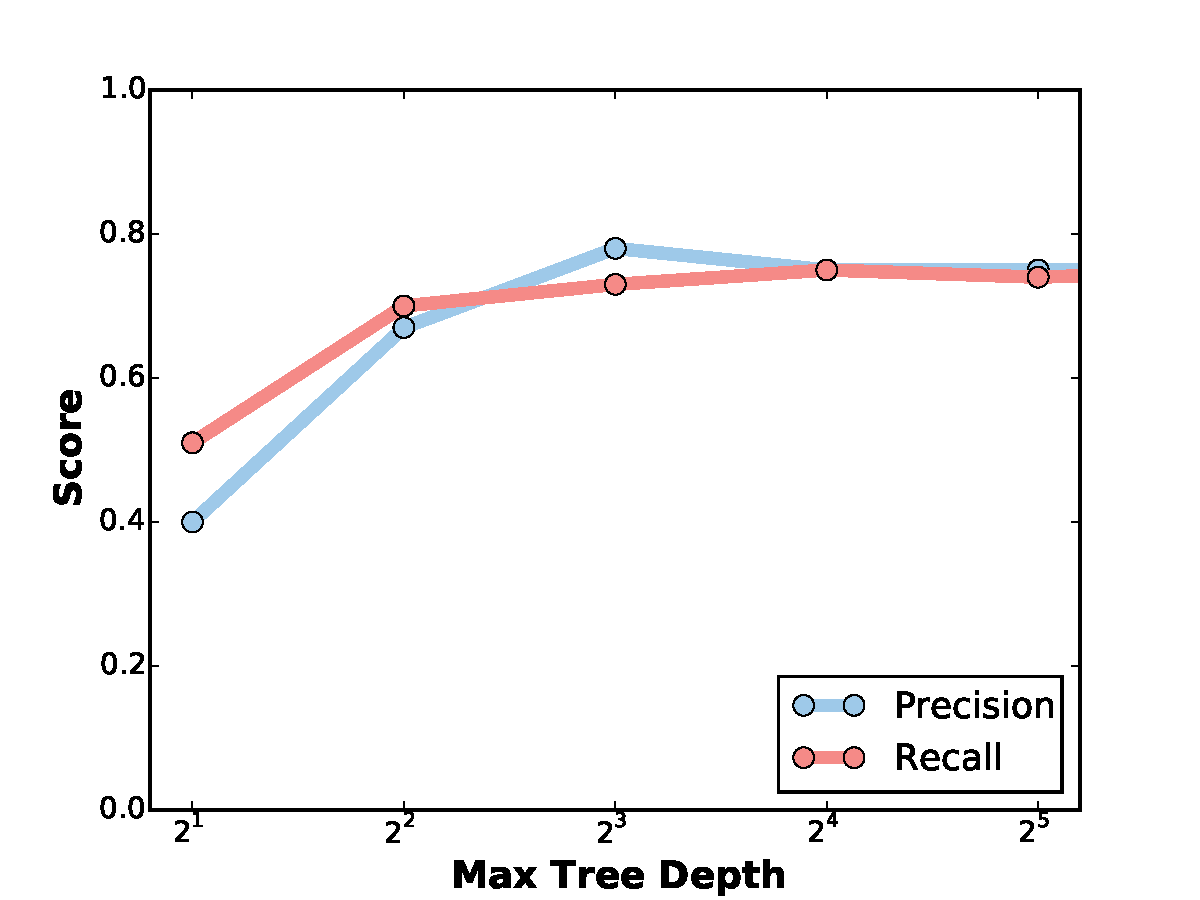
\includegraphics[width=0.7\linewidth]{figure/depth.pdf}
	\caption{Impact of max depth on the accuracy of the decision tree.}
\end{figure}

\begin{figure}[h!]
    \centering
	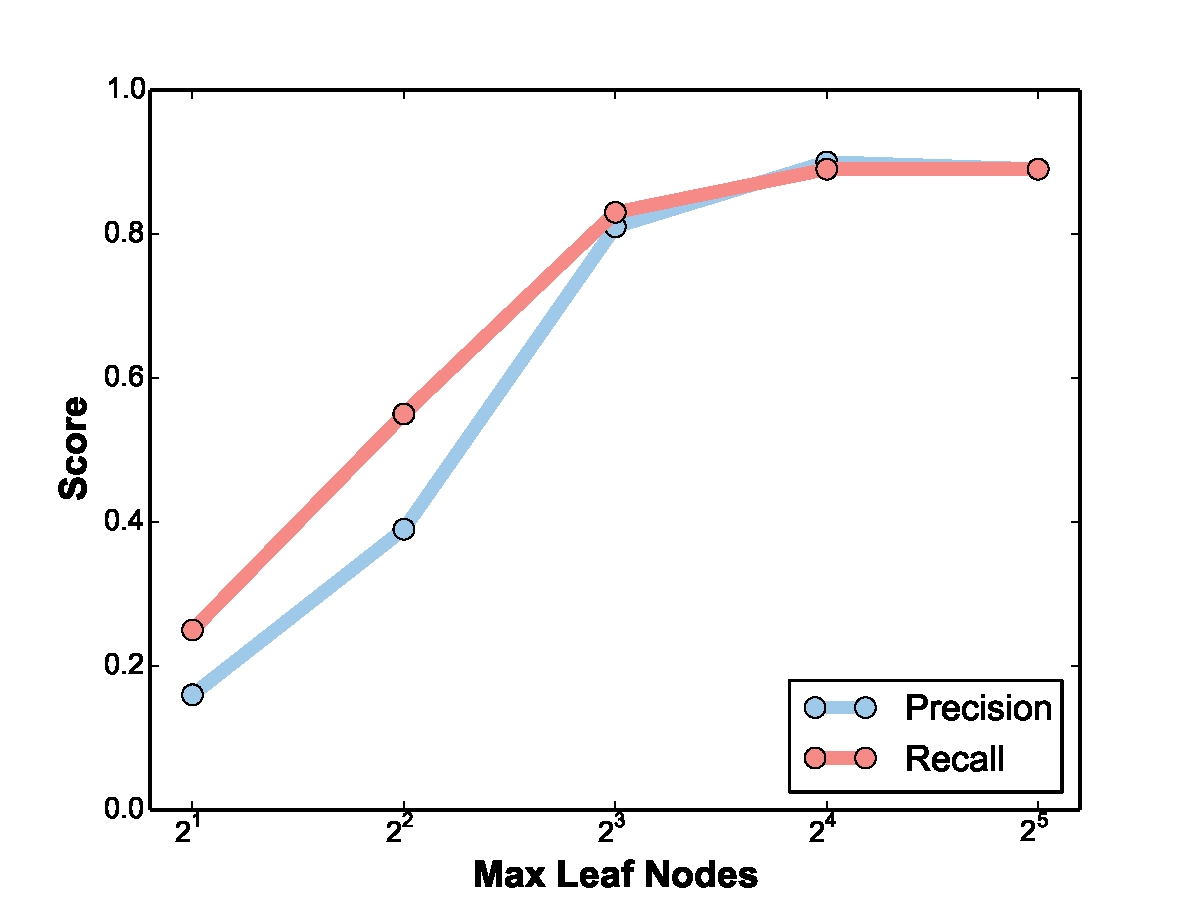
\includegraphics[width=0.7\linewidth]{figure/leaves.pdf}
	\caption{Impact of max leaf nodes on the accuracy of the decision tree.}
\end{figure}

\begin{table}[h!]
\centering
\small{
  \centering
  \begin{tabular}{l|llll} 
	\toprule
   		Class &  Precision  &  Recall &  F1-score  &  Support  \\    
    \midrule
		0.0   &    1.00   &   0.00   &   1.00   &     84   \\
        1.0   &    0.99   &   1.00   &   0.99   &     74   \\
        2.0   &    0.98   &   0.99   &   0.98   &     81   \\
        3.0   &    0.54   &   0.39   &   0.45   &     18   \\
        4.0   &    1.00   &   1.00   &   1.00   &     69   \\
        5.0   &    1.00   &   0.99   &   0.99   &     70   \\
        6.0   &    1.00   &   0.95   &   0.97   &     60   \\
        7.0   &    0.41   &   0.95   &   0.57   &     19   \\
        8.0   &    0.00   &   0.00   &   0.00   &     17   \\
        9.0   &    0.56   &   0.52   &   0.54   &     27   \\
    \midrule
Avg / Total   &    0.90   &   0.91   &   0.90   &    519   \\
   \bottomrule
   \end{tabular}
 }
%\nocaptionrule
\caption{Per-class accuracy of the default decision tree.}
\label{tab:dt_stats}
\end{table}



